% Chapter 3 -- structure from table of content.md; impersonal academic style; no shallow subsections

\reportchapter{3}{System Design and Architecture}{Design principles, data flows, ingestion and persistence models, and reasoning architecture.}

\section{Introduction}

This chapter translates the requirements defined in Chapter~2 into a concrete system design for the political Graph-RAG platform. The objective is to specify how evidence is acquired, structured, stored, retrieved, and synthesized without yet entering implementation-level code detail (Chapter~4) or empirical evaluation (Chapter~5). The presentation proceeds from design principles and refined use cases to data flows, ingestion architecture, knowledge representation, physical schemas, and the reasoning loop that connects hybrid retrieval to grounded answers.

\section{Design Principles}

Four principles guided architectural decisions throughout the PFE: separation of concerns, hybrid evidence representation, traceability by design, and evolvability with modularity. Together they ensure that each pipeline stage can be inspected, replaced, or extended independently while preserving analytical trust.

\textbf{Separation of concerns.} Acquisition, normalization, extraction, graph publication, vector indexing, retrieval, and synthesis are isolated into distinct services and storage roles. The frontend exposes analytical and administrative routes separately; the backend groups API endpoints by responsibility (ingestion, query, administration, health). Figure~\ref{fig:component-architecture} summarizes the major component boundaries and their interactions across the offline and online paths. Ingestion workers, extraction services, persistence connectors, and the reasoning engine communicate through well-defined interfaces rather than shared mutable state. This separation supports the modularity required by FR-09 and allows partial pipeline reruns when only one derived artifact changes.

\begin{figure}[H]
    \centering
    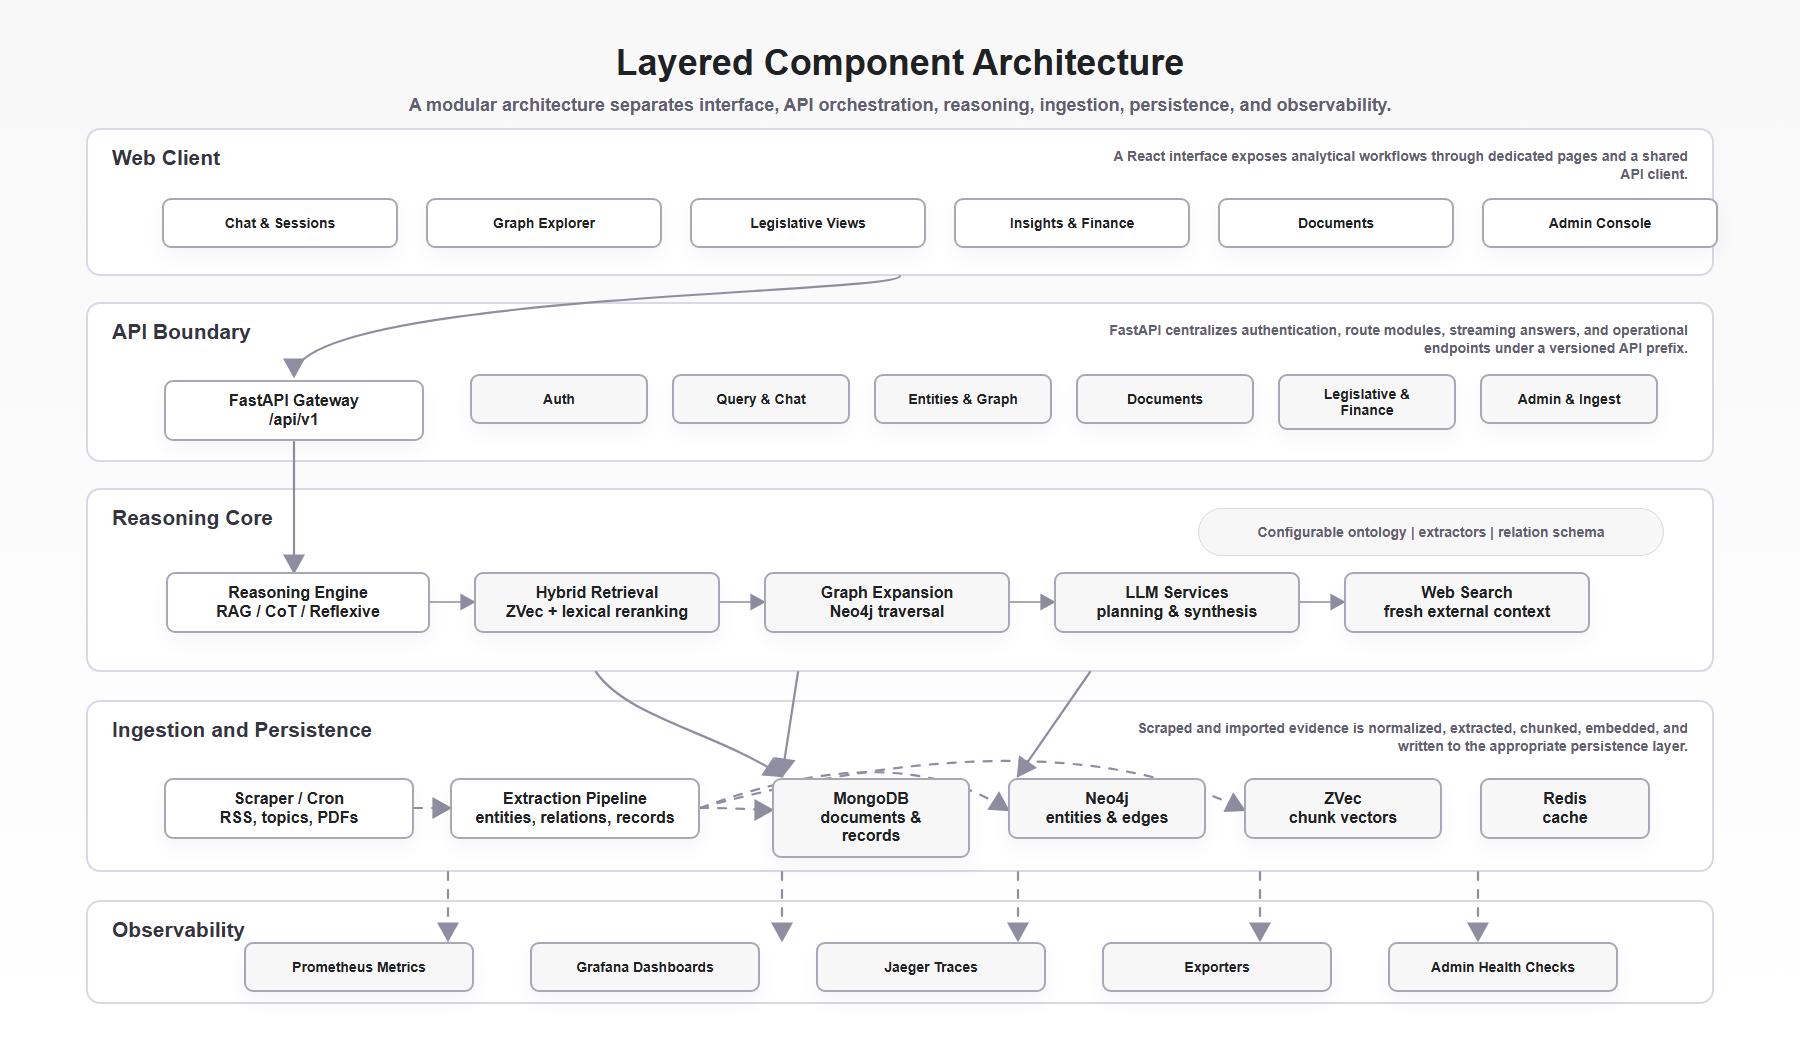
\includegraphics[width=0.96\textwidth,height=0.78\textheight,keepaspectratio]{images/component_architecture.png}
    \caption{Logical component architecture and separation of pipeline responsibilities.}
    \label{fig:component-architecture}
\end{figure}

\textbf{Hybrid evidence representation.} Political analysis requires both unstructured textual recall and structured relational precision. The design therefore maintains parallel representations: document-centric records and chunks for semantic search, canonical entities and typed edges for traversal, and structured analytical records (legislative, financial, conflict-oriented) where schema-specific views add value. Figure~\ref{fig:vector-vs-graph} contrasts the roles of vector space and graph space in the same query workflow. Vector retrieval contributes topical similarity and passage-level grounding; graph traversal contributes entity disambiguation, multi-hop paths, and temporal constraints. Neither store alone satisfies FR-04; the reasoning layer must fuse evidence from both modalities before synthesis (FR-07).

\begin{figure}[H]
    \centering
    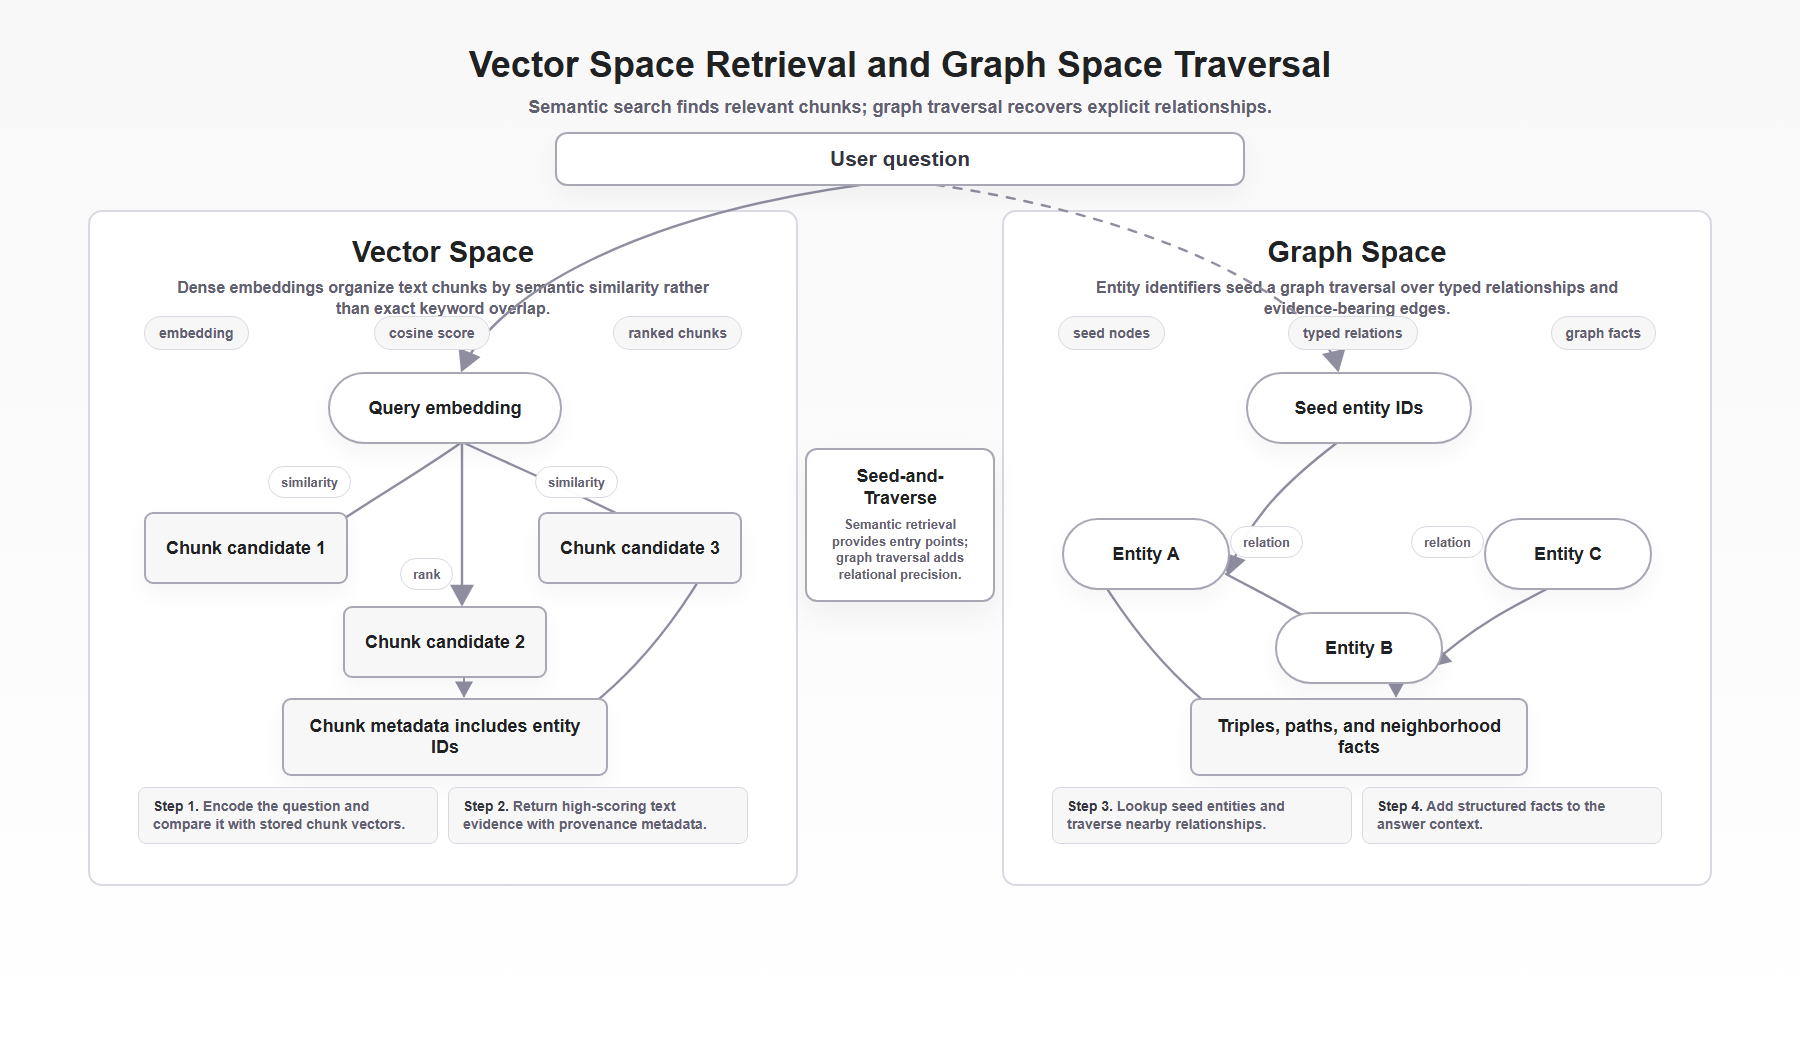
\includegraphics[width=0.96\textwidth,height=0.78\textheight,keepaspectratio]{images/vector_vs_graph_spaces.png}
    \caption{Complementary roles of vector retrieval and graph traversal in hybrid evidence access.}
    \label{fig:vector-vs-graph}
\end{figure}

\textbf{Traceability by design.} Every analytical output must remain linked to inspectable artifacts: source documents, chunk identifiers, graph nodes and edges used in traversal, and reasoning-step metadata exposed in the interface. Traceability is enforced at the data-model level (provenance fields on documents and assertions) and at the reasoning level (cited spans, graph-fact references, and optional audit loops in reflexive mode). This principle implements the validation criteria for reasoning and observability defined in Chapter~2.

\textbf{Evolvability and modularity.} Domain ontologies, extraction prompts, source connectors, and embedding settings may evolve during the internship and in later deployments. The architecture therefore treats MongoDB documents as the system of record for raw evidence and processing checkpoints, while Neo4j and ZVec hold derived views that can be rebuilt from documents without re-scraping sources. Containerized services and horizontal scaling of stateless workers (ingestion, API, reasoning) support growth in corpus size without redesigning the logical topology illustrated in Figure~\ref{fig:system-component-overview}. Observability (metrics, logs, traces) is treated as a cross-cutting concern rather than an afterthought, consistent with the non-functional requirements on auditability and operational diagnosis.

\begin{figure}[H]
    \centering
    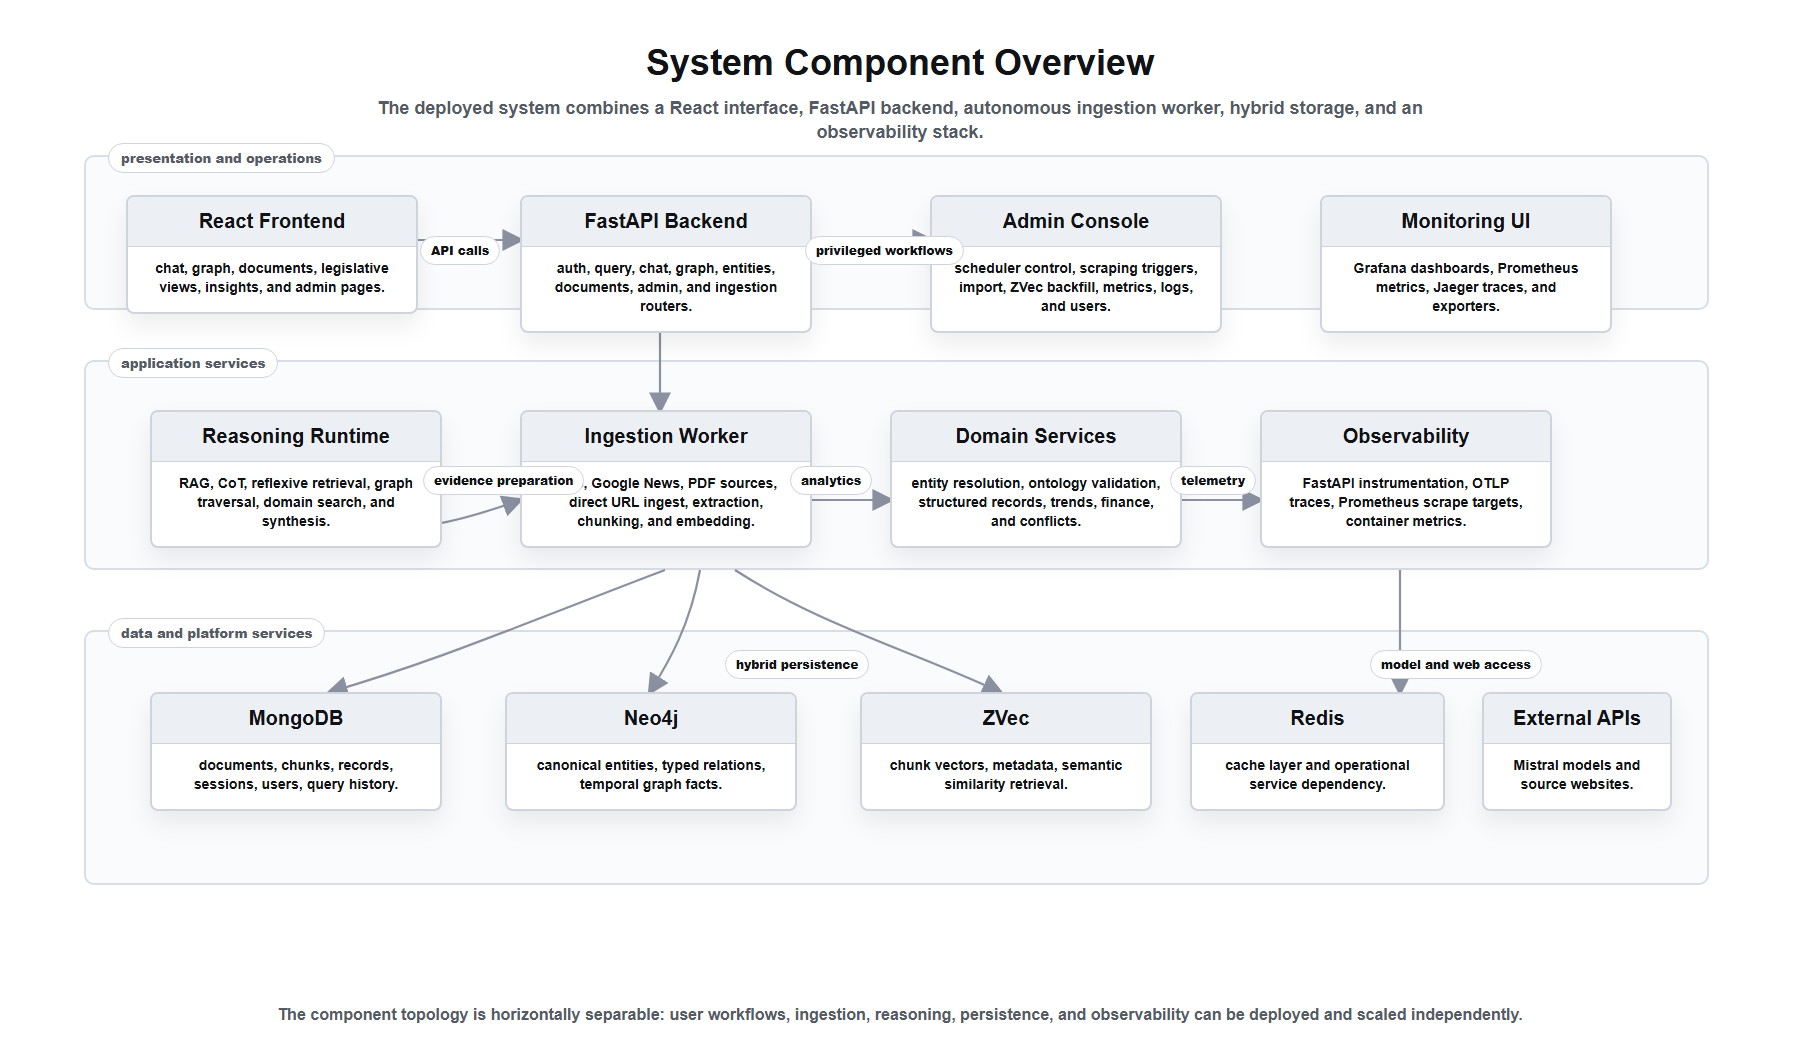
\includegraphics[width=0.96\textwidth,height=0.78\textheight,keepaspectratio]{images/system_component_overview.png}
    \caption{System component overview for ingestion, persistence, reasoning, and observability.}
    \label{fig:system-component-overview}
\end{figure}

\section{Use Case Refinement}

Chapter~2 introduced actors and primary use cases at requirement level. The detailed model refined here guided API and frontend boundaries. Authenticated users interact through cited question answering (with selectable reasoning depth), chat history, graph exploration, document library consultation, legislative and financial dashboards, trend and conflict views, and entity comparison. Each analytical workflow consumes prepared evidence from MongoDB, Neo4j, and ZVec rather than triggering full ingestion at query time; live web supplementation applies only when configured for recent events not yet indexed locally.

The system administrator supervises scheduler configuration, scraping and backfill jobs, ingestion log inspection, user management, health metrics, and selective reindexing of derived artifacts. Operational routes are isolated from standard analytical navigation through role-based access control in the frontend and privileged backend endpoints, so infrastructure actions are not conflated with everyday analytical sessions. Access control is modeled as a strict boundary between \emph{user} and \emph{administrator} roles: analytical capabilities require authentication, while administrative capabilities require an elevated role verified on both client and server.

Figure~\ref{fig:detailed-use-case} formalizes the use cases attached to each side of this boundary and aligns them with the implemented route structure. The model clarifies that graph exploration and document inspection are peer workflows to chat-based questioning, not secondary features. Administrative use cases (scheduler control, scraping supervision, reindexing) operate on the same evidence pipeline but must not bypass quality gates or idempotency rules defined for ingestion.

\begin{figure}[H]
    \centering
    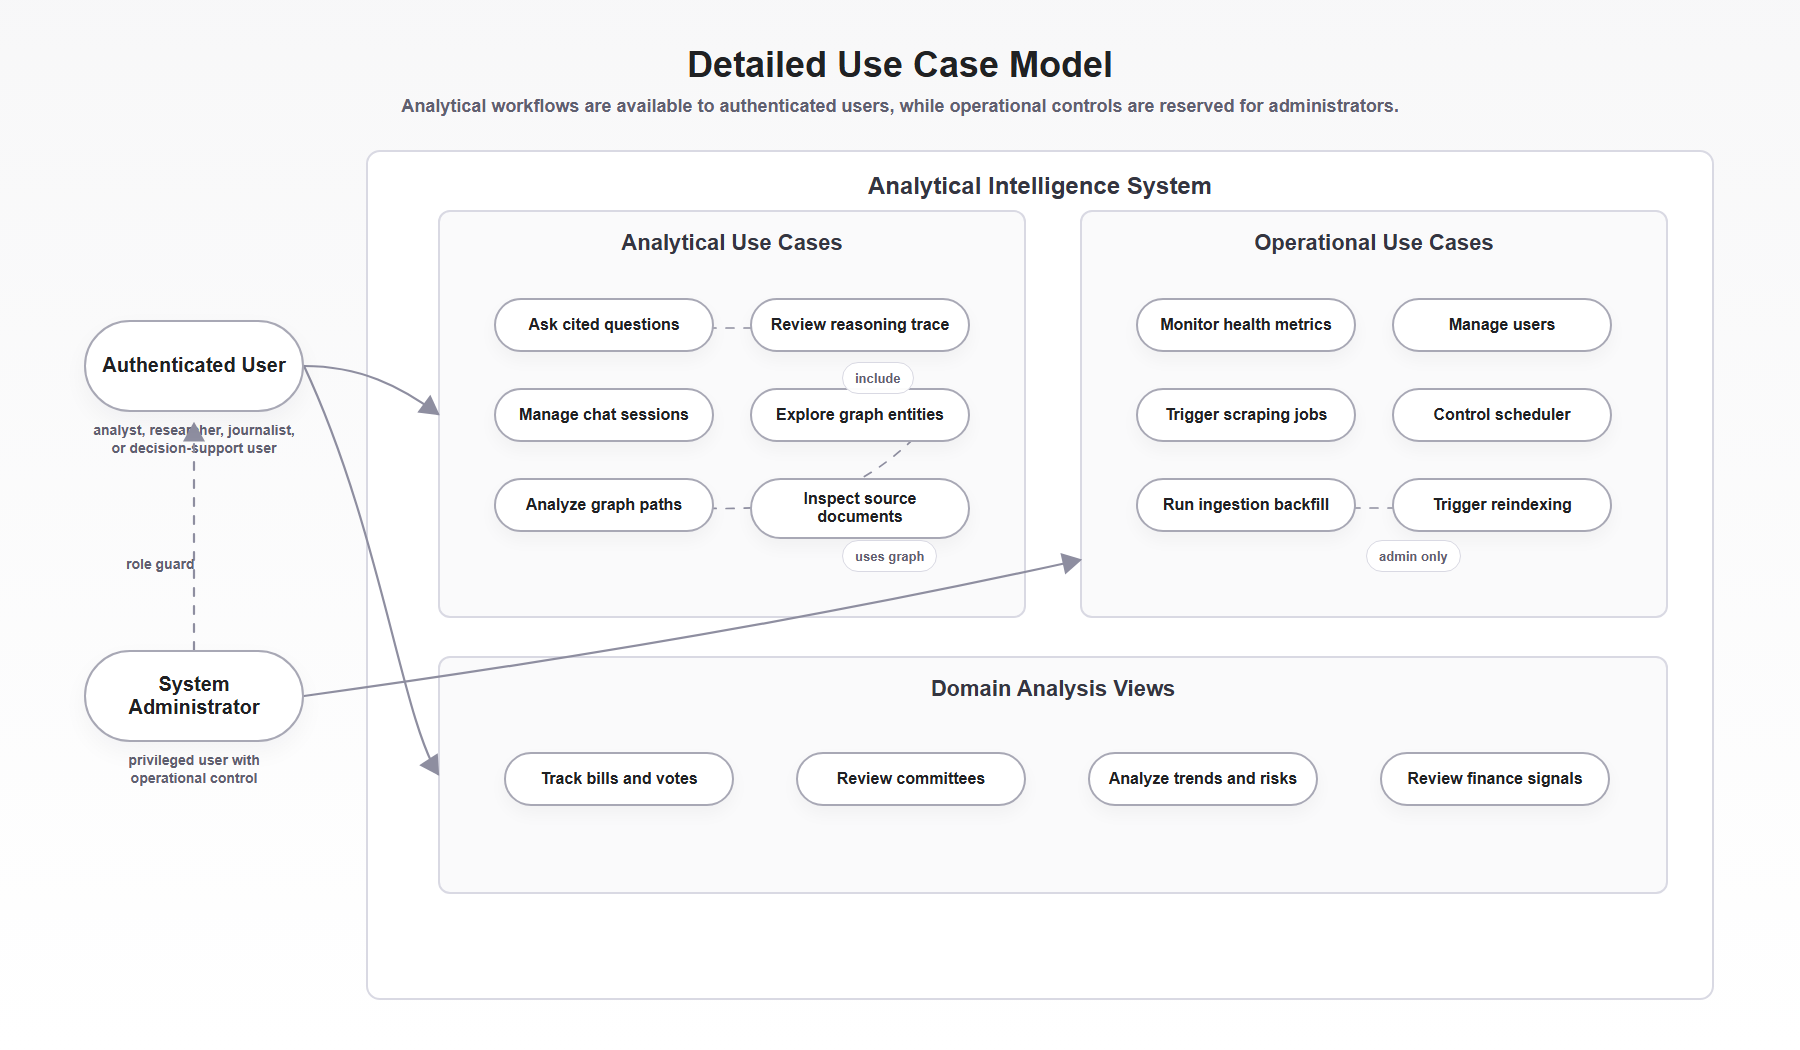
\includegraphics[width=0.96\textwidth,height=0.78\textheight,keepaspectratio]{images/detailed_use_case.png}
    \caption{Detailed use case model for analytical and administrative workflows.}
    \label{fig:detailed-use-case}
\end{figure}

\section{Data Flow Architecture}

The platform distinguishes \textbf{offline} evidence construction from \textbf{online} query-time reasoning. Offline flows prepare documents, structured records, graph topology, and vectors; online flows consume those artifacts under latency constraints suitable for interactive analysis.

External sources (RSS feeds, web articles, Google News topics, direct URLs, PDF reports) enter through the acquisition layer and are normalized into MongoDB documents with source metadata and processing flags. Quality gating rejects unsuitable content before extraction. Accepted documents pass through graph extraction (entities and relations to Neo4j; mentions and assertions in MongoDB), structured extraction (domain records such as bills, votes, committees, contributions, conflict flags), and chunking with embedding into ZVec. Checkpoint flags on each document make the offline sequence resumable and idempotent.

At query time, a request arrives at the FastAPI endpoint with parameters for reasoning mode, hop limit, and optional web search. The reasoning engine retrieves ZVec chunks and Neo4j paths (and structured records when the planner requests them), fuses evidence, and invokes synthesis with citation metadata. The response returns answer text, sources, graph facts, traces, and confidence signals for the frontend. Online flow does not mutate the corpus except through explicit administrative ingestion triggers.

Figure~\ref{fig:data-flow-diagram} consolidates both paths from external sources to cited answers. The diagram emphasizes responsibility splits: MongoDB holds documents and derived textual artifacts; Neo4j holds canonical relational topology; ZVec holds embedded chunks linked to document and entity identifiers. Query execution reads from all three stores but writes only to session and history collections unless an administrator launches ingestion.

\begin{figure}[H]
    \centering
    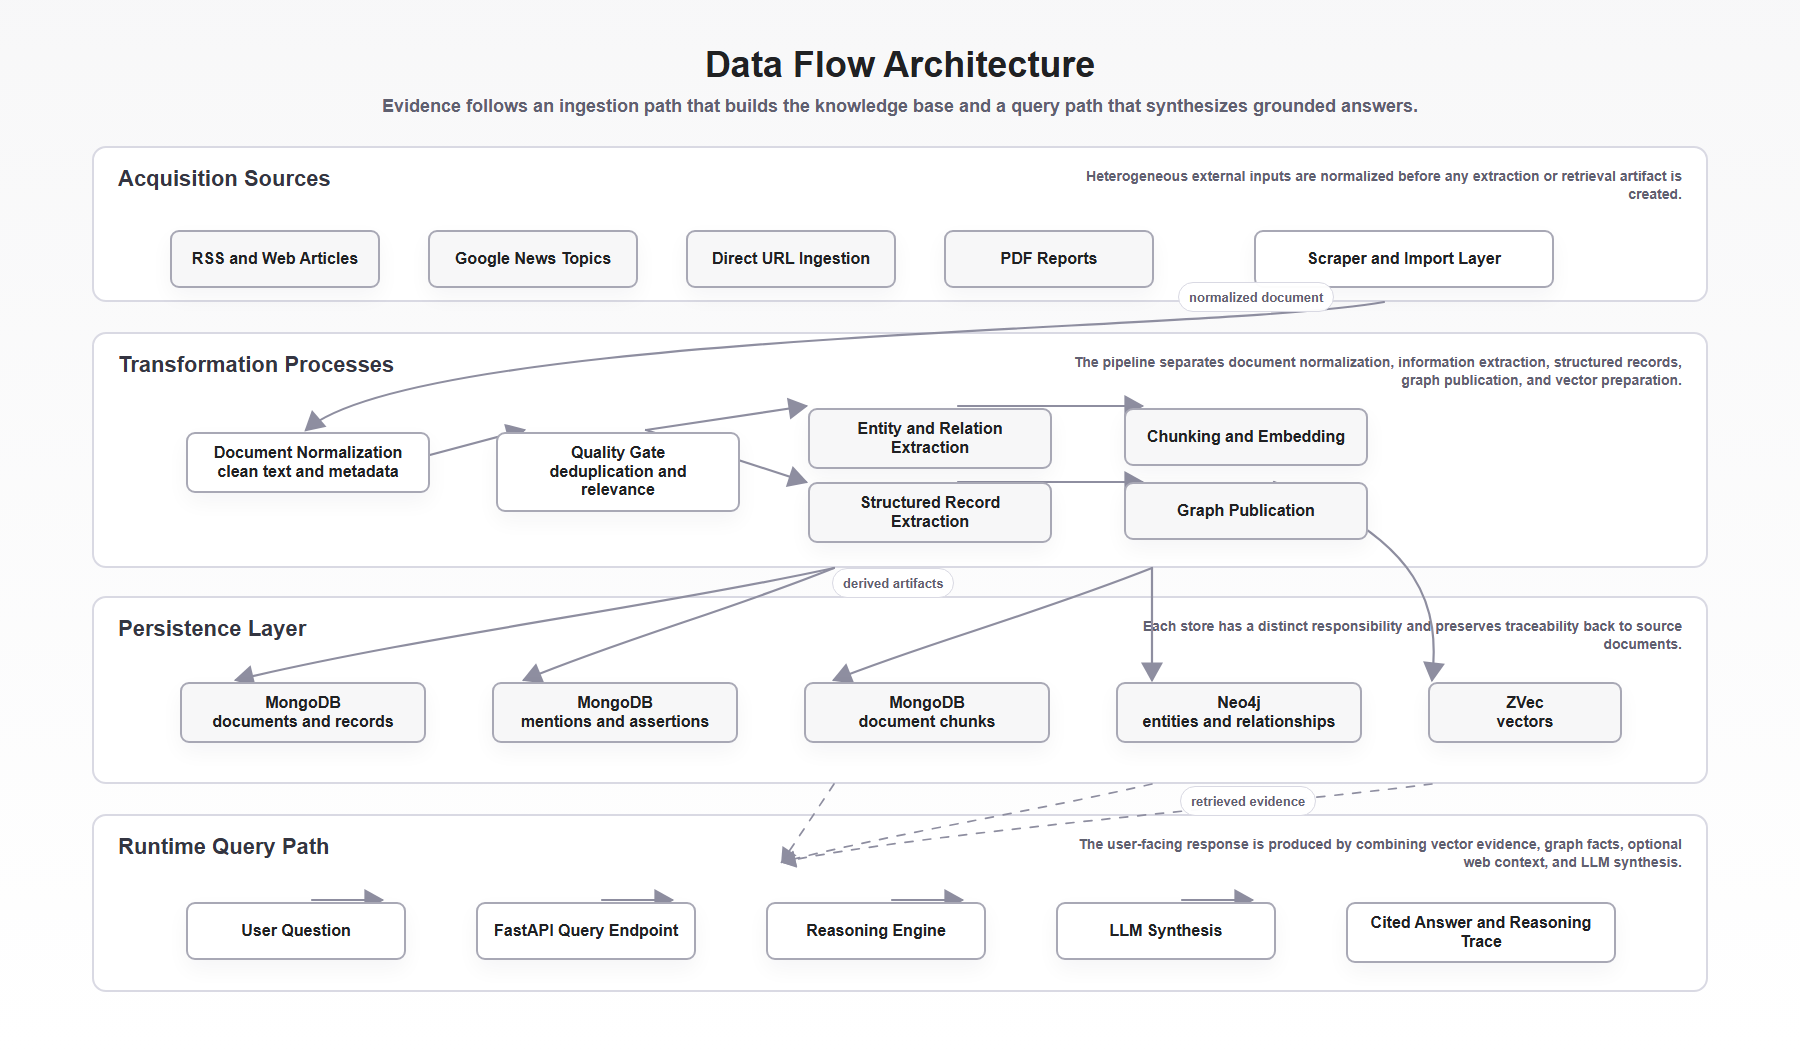
\includegraphics[width=0.96\textwidth,height=0.78\textheight,keepaspectratio]{images/data_flow_diagram.png}
    \caption{Data flow architecture from acquisition to grounded answer generation.}
    \label{fig:data-flow-diagram}
\end{figure}

\section{Ingestion Architecture}

Ingestion implements FR-01, FR-08, FR-09, and FR-10 through a multi-level acquisition strategy, explicit normalization and quality gates, and a document-level state machine.

The ingestion engine combines three complementary levels rather than a single crawler template. \textbf{Level~1} monitors a curated registry of \textbf{57 high-precision outlets} on schedules (RSS, institutional portals, known political feeds). \textbf{Level~2} extends coverage with query-driven deep discovery for thematic gaps (search, link traversal, dynamic rendering, pagination). \textbf{Level~3} handles unstructured documents such as PDF reports through high-fidelity parsers that preserve layout and tables. Figure~\ref{fig:autonomous-crawler-final} summarizes the pipeline from collection to retrieval-ready artifacts. Discovery, extraction, normalization, and quality control remain separate stages so new source families can be added without rewriting the reasoning engine.

\begin{figure}[H]
    \centering
    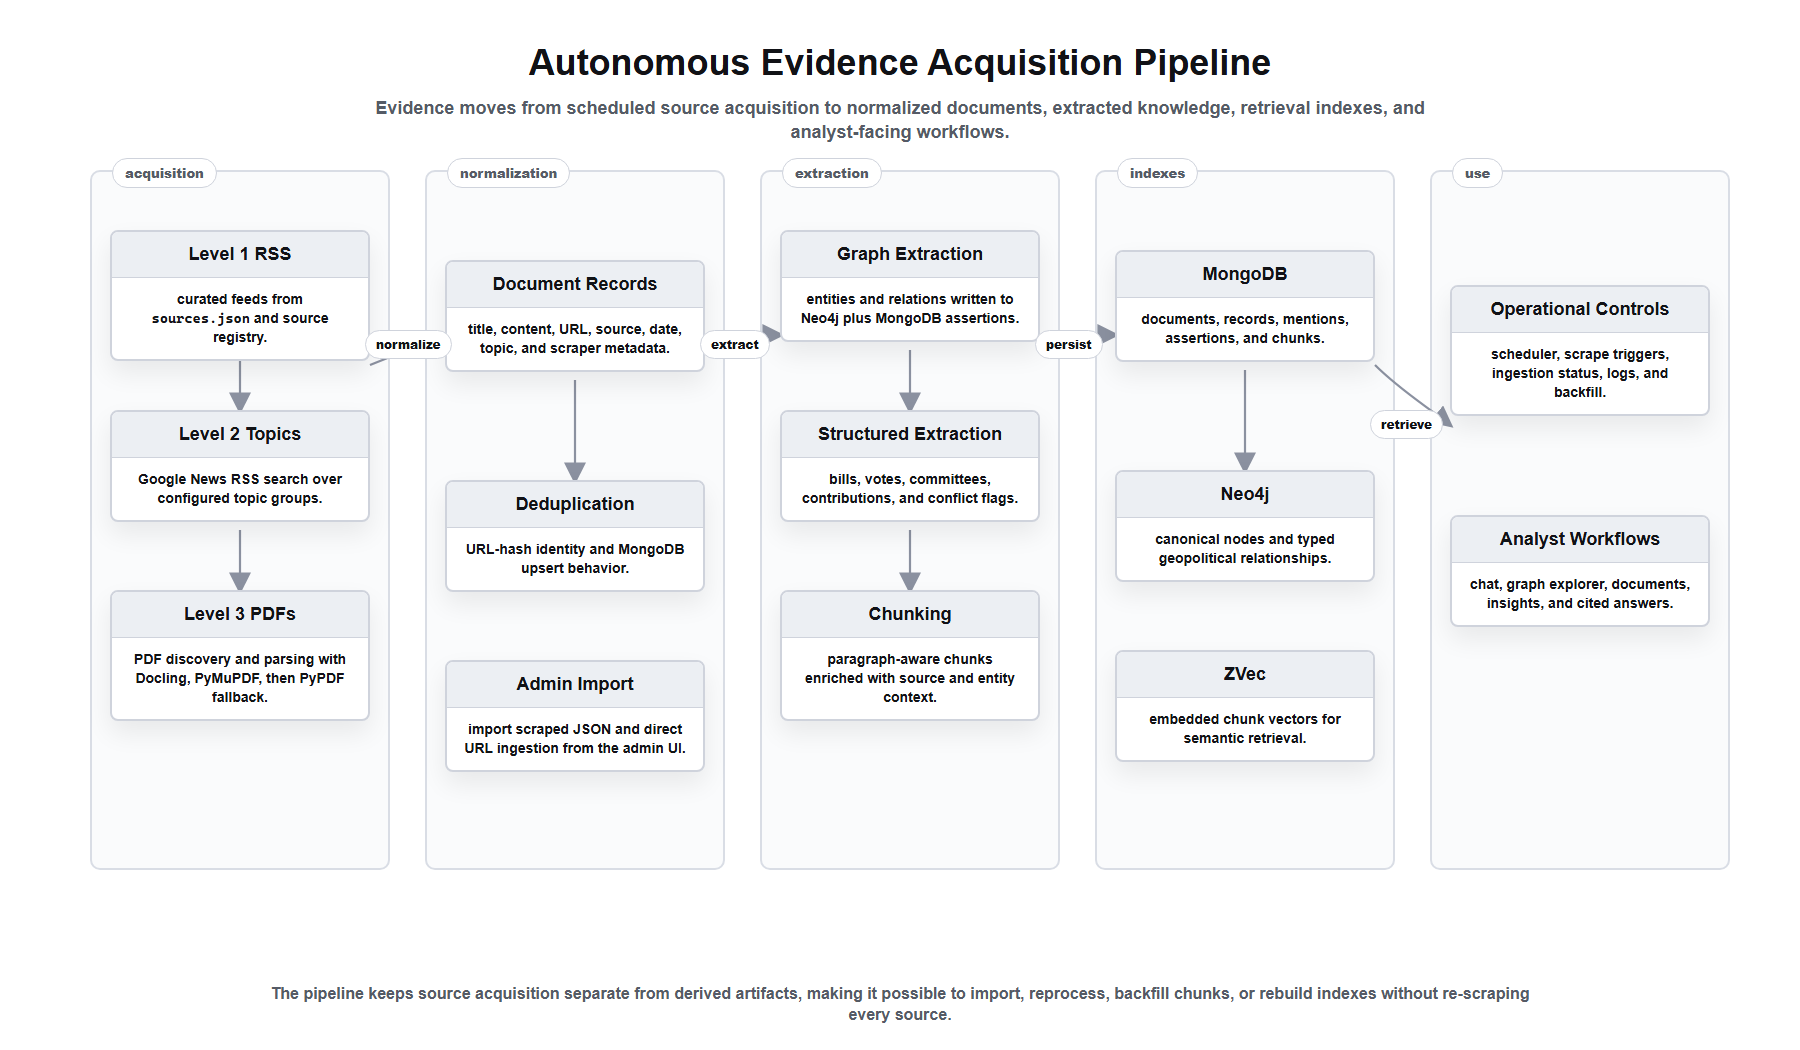
\includegraphics[width=0.96\textwidth,height=0.78\textheight,keepaspectratio]{images/autonomous_crawler_pipeline.png}
    \caption{Autonomous evidence acquisition pipeline from source collection to retrieval-ready artifacts.}
    \label{fig:autonomous-crawler-final}
\end{figure}

All acquired content converges on a unified document schema: identifiers, timestamps, provenance, language hints, and normalized body text. Quality gates filter documents whose length, metadata, or topical signal fall below thresholds for reliable extraction; rejected items remain logged for administrator review without polluting graph or vector indexes. Normalization is the prerequisite for deduplication and for consistent joint extraction (FR-02).

The document lifecycle is modeled as an explicit state machine with checkpoints rather than a monolithic ingest operation. Flags such as \texttt{graph\_extracted}, \texttt{structured\_extracted}, and \texttt{chunks\_created} record completion of each derived stage so that partial reprocessing is possible when prompts, schemas, or embeddings change. Figure~\ref{fig:state-document-lifecycle} shows transitions from raw acquisition through quality gating to graph publication, structured records, and vector indexing. Explicit states improve operational control: the pipeline can resume after interruption, skip completed work, or rebuild only derived layers without re-scraping originals.

\begin{figure}[H]
    \centering
    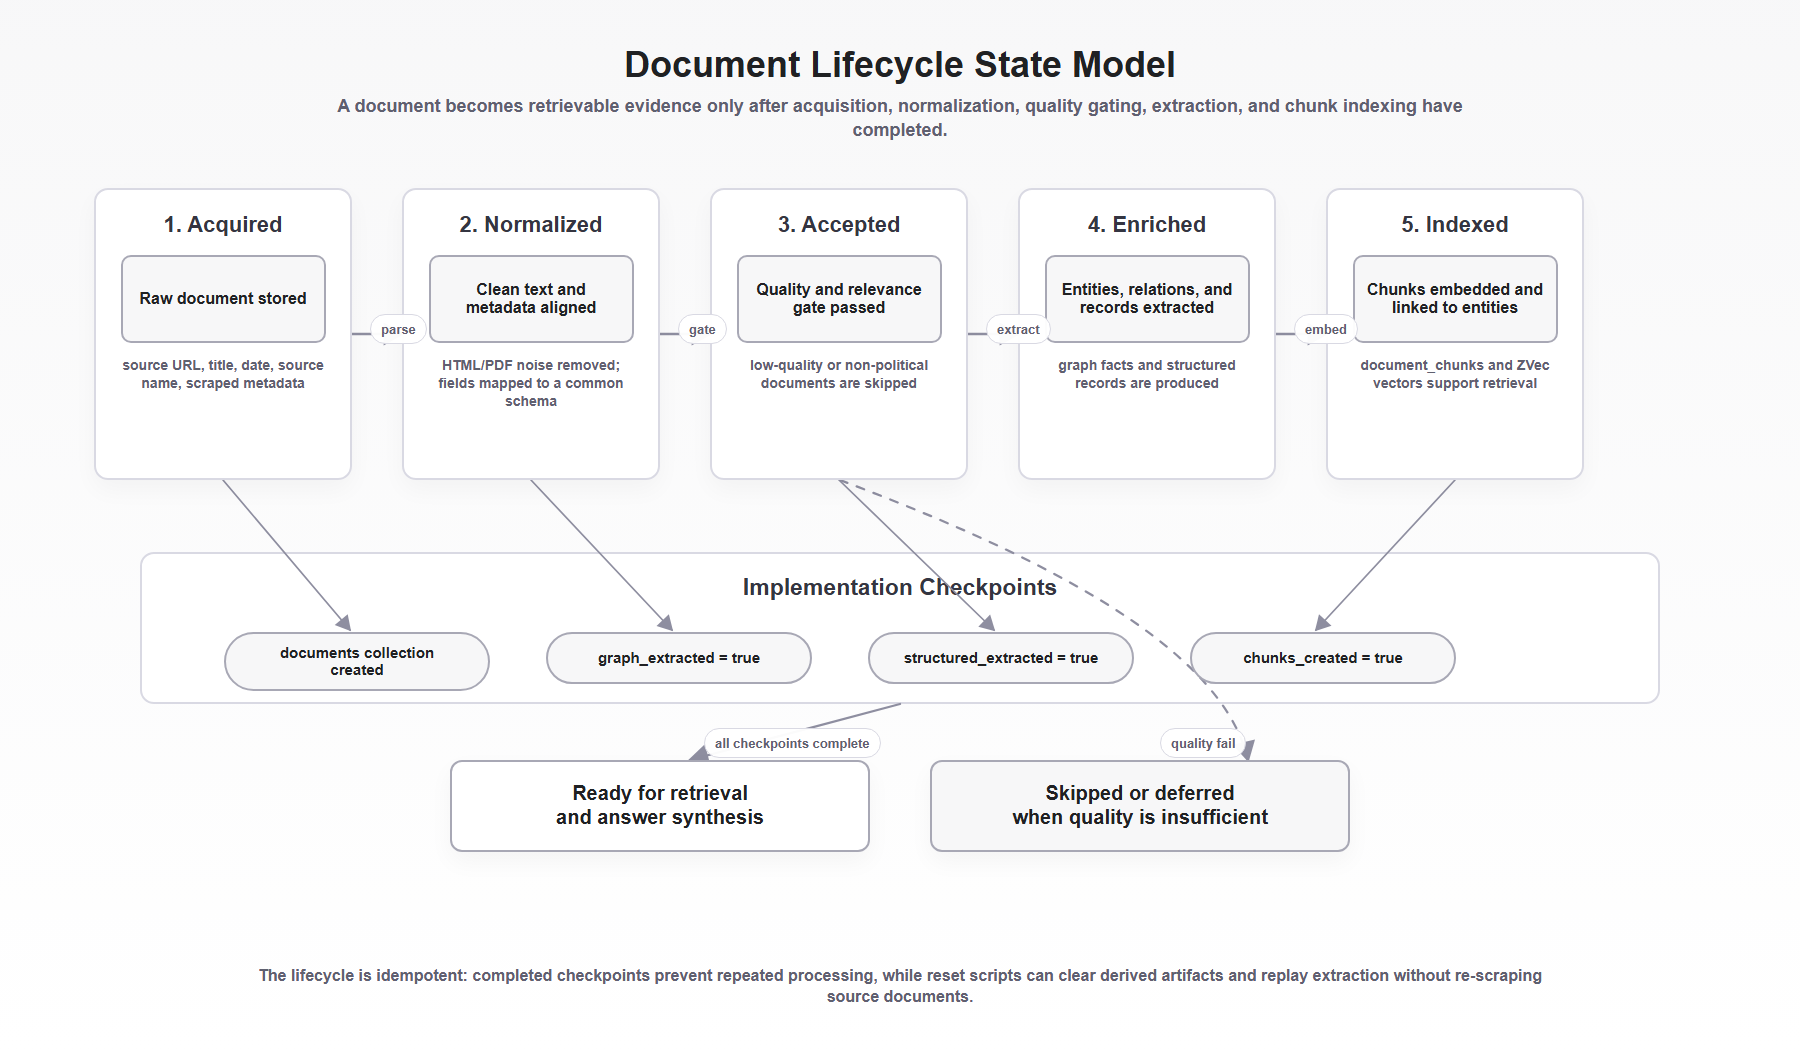
\includegraphics[width=0.96\textwidth,height=0.78\textheight,keepaspectratio]{images/state_document_lifecycle.png}
    \caption{Document lifecycle and ingestion checkpoints before retrieval.}
    \label{fig:state-document-lifecycle}
\end{figure}

\section{Knowledge Representation and Ontology}

The knowledge layer centers on a geopolitical property graph supplemented by document-grounded structured records and vectorized chunks.

The Neo4j ontology defines canonical node types including \texttt{POLITICIAN}, \texttt{PARTY}, \texttt{ORGANIZATION}, \texttt{INSTITUTION}, \texttt{EVENT}, and related geopolitical categories. Approximately \textbf{32 typed relation families} cover actor ties, geopolitical links, events, financial or influence relations, and evidence-backed assertions. Entity resolution maps surface mentions to stable canonical identifiers so syndicated or variant spellings do not fragment the graph. Figure~\ref{fig:class-domain-model} links graph topology to MongoDB evidence objects and ZVec chunks: bills, votes, contributions, and conflict flags remain document-grounded structured data in MongoDB, while actors, institutions, places, and events form traversable graph structure in Neo4j.

\begin{figure}[H]
    \centering
    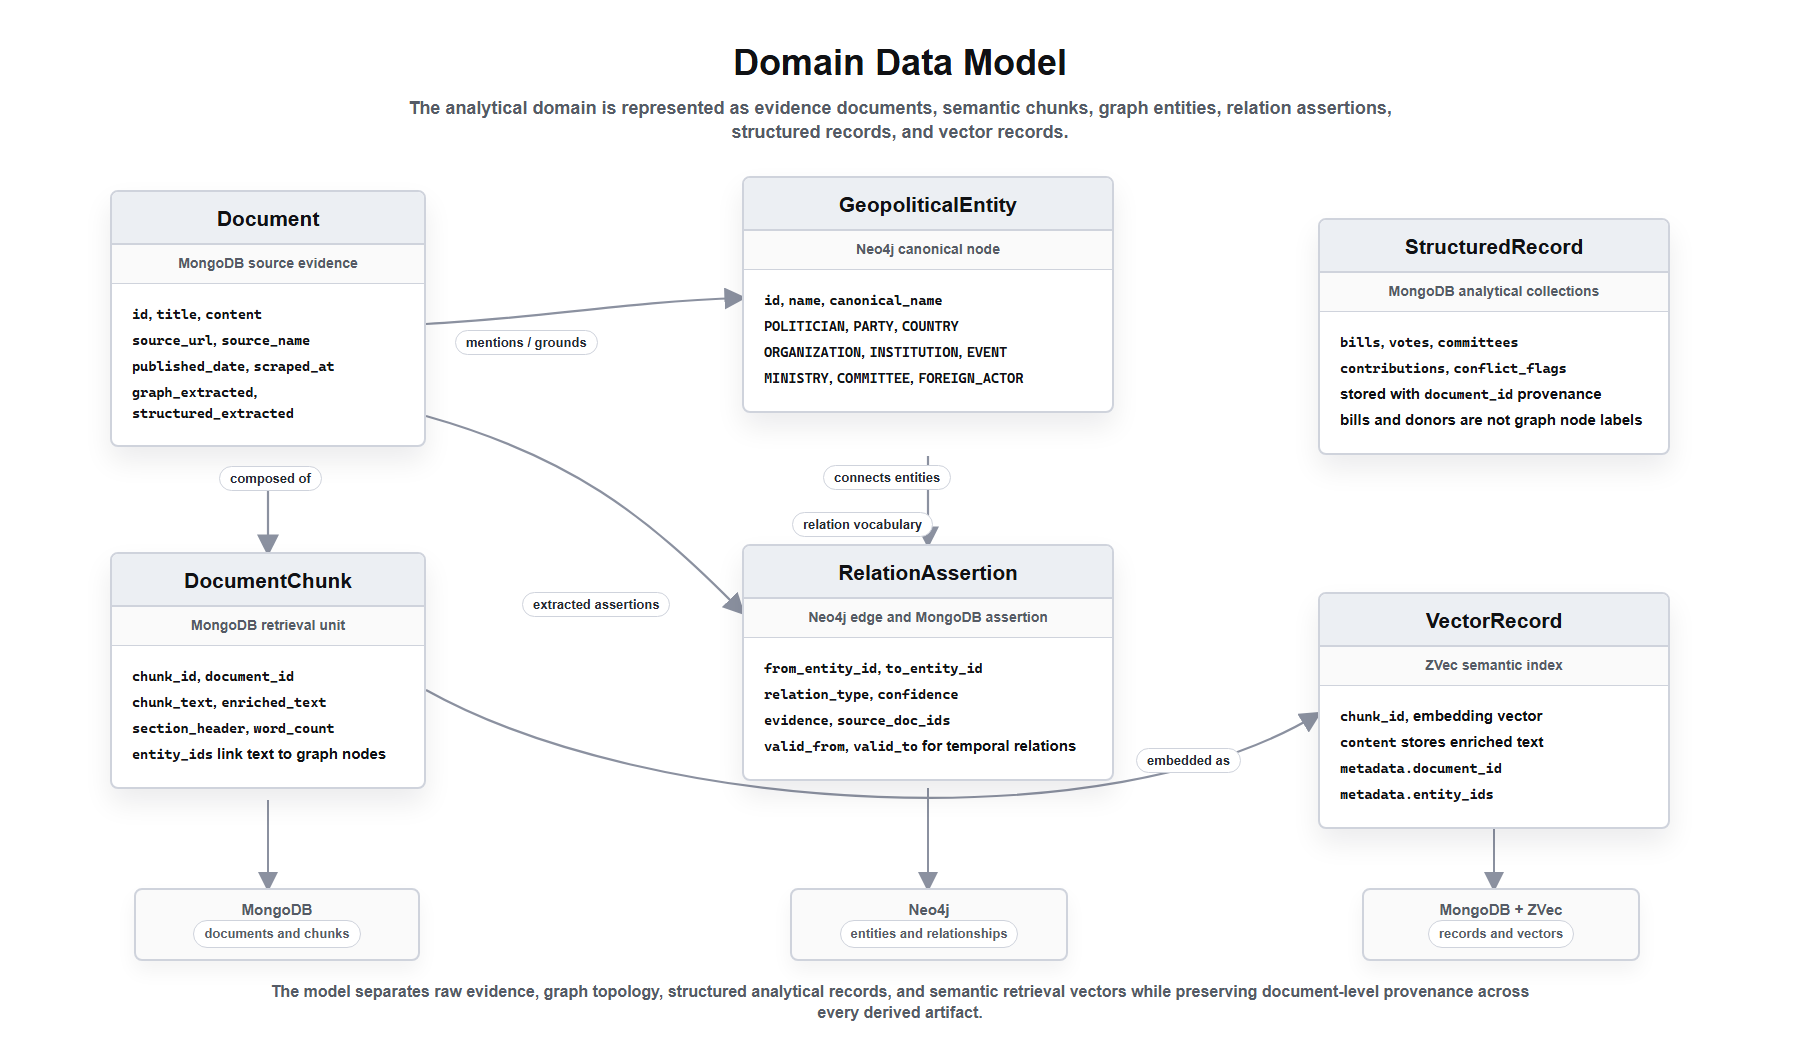
\includegraphics[width=0.96\textwidth,height=0.78\textheight,keepaspectratio]{images/class_domain_model.png}
    \caption{Domain data model linking evidence, graph topology, structured records, and vector retrieval.}
    \label{fig:class-domain-model}
\end{figure}

Political relations are time-bounded: office holding, alliances, and opposition change with elections, conflicts, and institutional reform. Where chronology is available, edges carry \texttt{valid\_from} and \texttt{valid\_to} attributes so queries can reconstruct states valid at a requested period rather than mixing obsolete and current facts. Temporal attributes support trend, conflict, and comparative use cases from Chapter~2 and condition multi-hop answers on FR-06.

Provenance is anchored on the \texttt{documents} collection: each chunk, mention, assertion, and structured record references its source document and extraction pass. Graph edges in Neo4j remain traceable to assertions stored in MongoDB before publication. This dual linkage satisfies traceability by design and enables the citation layer in the reasoning architecture.

\section{Data Model and Physical Schema}

Persistence is deliberately polyglot: a document store for evidence and operational metadata, a graph store for relational traversal, and a vector store for semantic recall.

MongoDB is the system of record for raw and derived textual evidence. Core collections include \texttt{documents} (provenance and processing state), \texttt{document\_chunks}, entity \texttt{mentions}, relation \texttt{assertions}, and domain-specific structured collections (legislative, financial, conflict). Application collections (\texttt{users}, chat \texttt{sessions}, \texttt{messages}, query \texttt{history}) are separated from evidence collections so that user activity does not complicate corpus rebuilds. Figure~\ref{fig:graph-vs-relational} motivates the document-centric primary store versus graph specialization: document storage preserves full text, extraction artifacts, and flexible schemas for heterogeneous political sources, while the graph store optimizes typed traversal and disambiguation rather than replacing document provenance.

\begin{figure}[H]
    \centering
    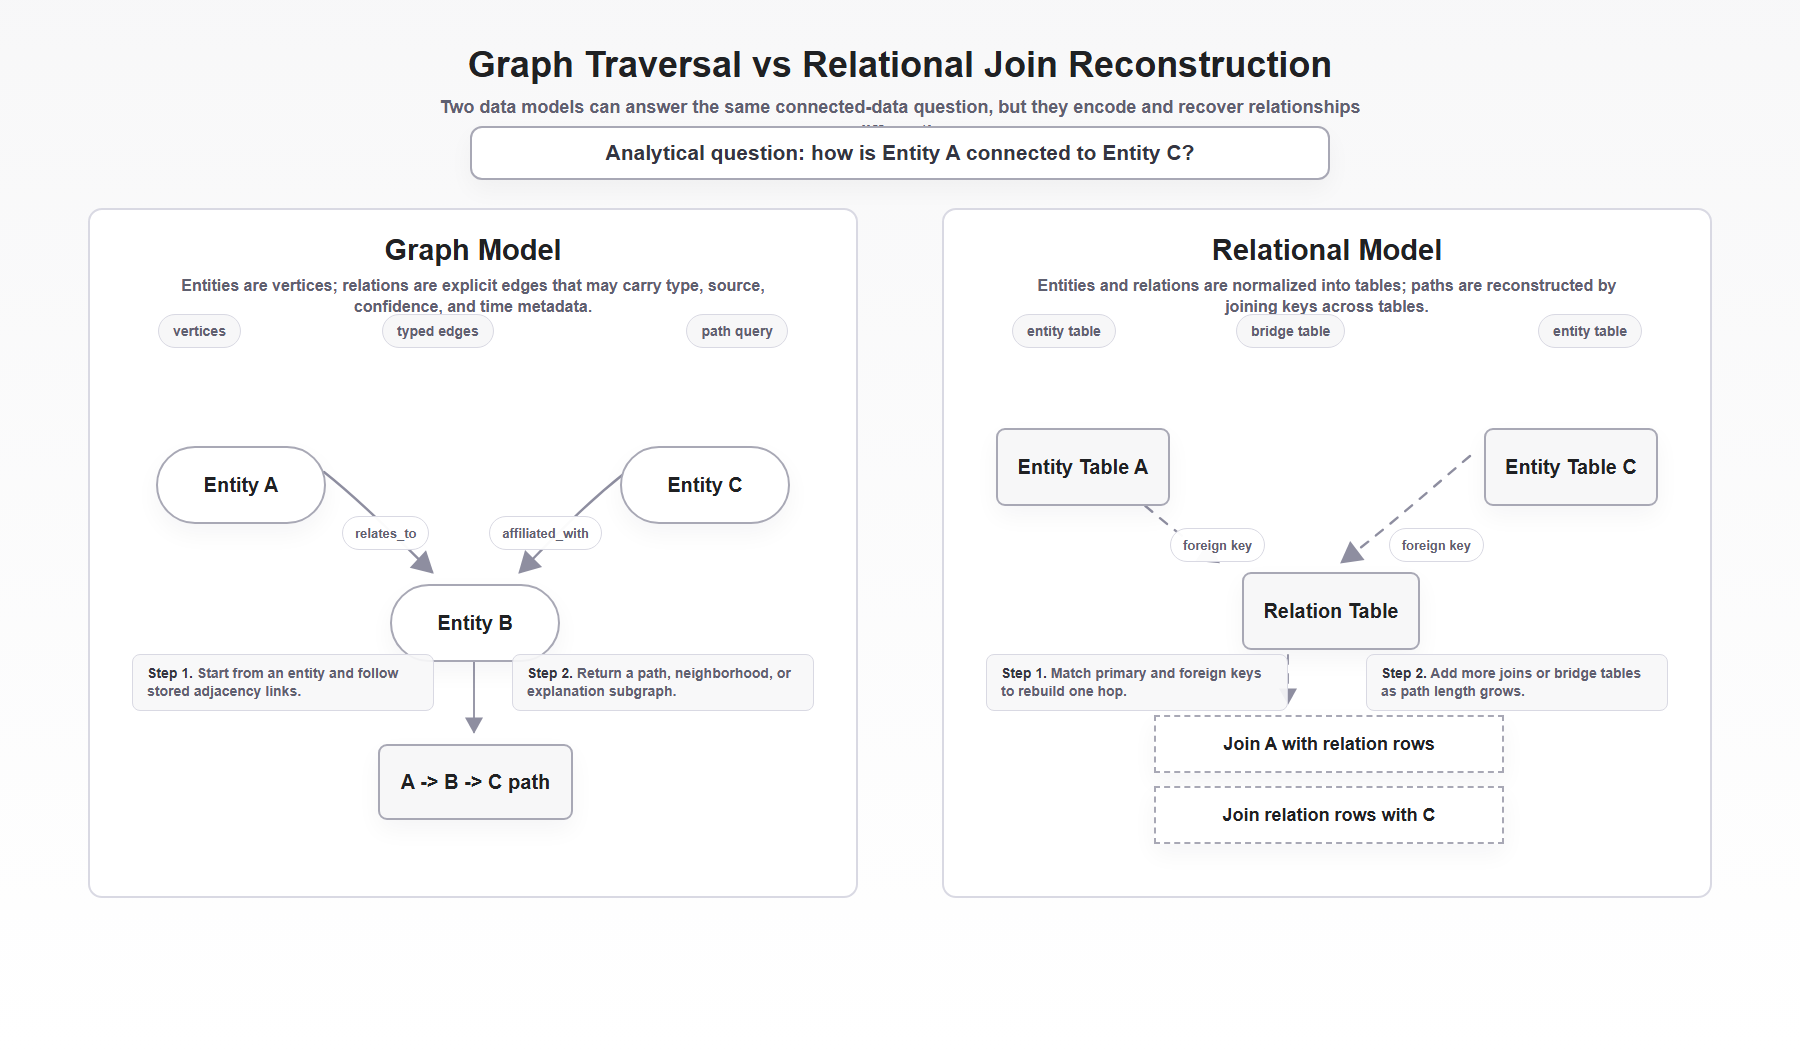
\includegraphics[width=0.96\textwidth,height=0.78\textheight,keepaspectratio]{images/graph_vs_relational.png}
    \caption{Document-centric evidence storage versus graph-native relational queries.}
    \label{fig:graph-vs-relational}
\end{figure}

Neo4j holds canonical entities and typed relationships produced after resolution and validation. The schema is optimized for multi-hop queries up to the performance target defined in Chapter~2 (approximately three hops under nominal load). Indexes and relationship types align with the ontology categories above; temporal attributes are applied on edges when evidence supports interval bounds.

ZVec stores dense embeddings of \texttt{document\_chunks} with metadata linking chunk identifiers, document identifiers, and associated entity identifiers where available. Vector records enable semantic recall in hybrid search (FR-04) and feed the first hop of standard RAG mode. Re-embedding can be executed independently of graph republication when only the embedding model changes.

Figure~\ref{fig:database-erd} presents the integrated physical view across MongoDB, Neo4j, and ZVec, including runtime collections for authentication and chat. The ERD clarifies that \texttt{documents} sit at the center of provenance links to chunks, structured records, and extraction artifacts, while Neo4j and ZVec remain rebuildable derived stores.

\begin{figure}[H]
    \centering
    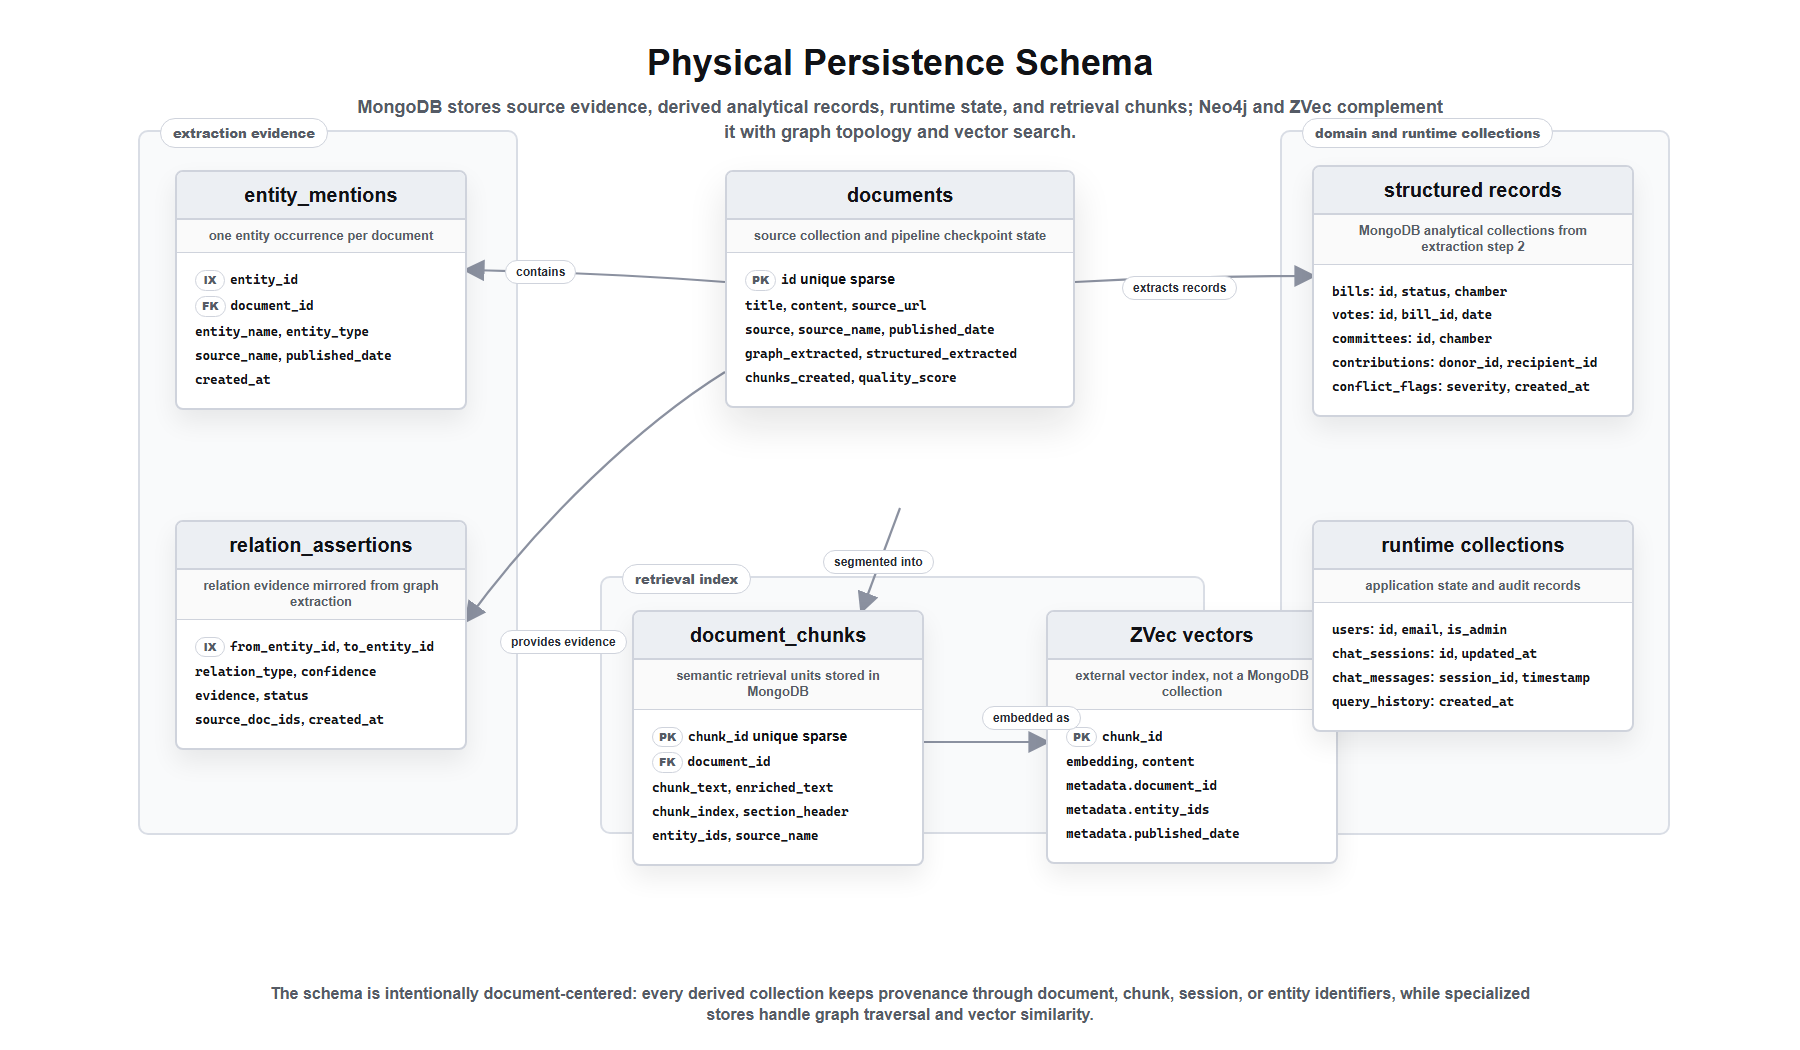
\includegraphics[width=0.96\textwidth,height=0.78\textheight,keepaspectratio]{images/database_erd.png}
    \caption{Physical persistence schema across MongoDB, Neo4j, and ZVec.}
    \label{fig:database-erd}
\end{figure}

\section{Reasoning Architecture}

The reasoning layer implements FR-04, FR-05, and FR-07 through a plan--retrieve--synthesize loop with selectable modes and explicit evidence fusion.

At design level, each query iteration performs three stages. \textbf{Planning} interprets the question and, in multi-hop modes, decomposes sub-questions or selects seed entities. \textbf{Retrieval} fetches ZVec chunks, Neo4j paths, and optional structured records. \textbf{Synthesis} generates a cited answer from fused context. Reflexive mode adds an audit step that tests evidence sufficiency and may trigger additional hops up to \textbf{MAX\_HOPS = 3}. Optional live web search supplements the local corpus when configured for breaking events not yet ingested. Figure~\ref{fig:sequence-reasoning} shows interactions among the API, reasoning engine, persistence stores, and language model; the loop terminates when acceptance criteria for the selected mode are met or the hop limit is reached.

\begin{figure}[H]
    \centering
    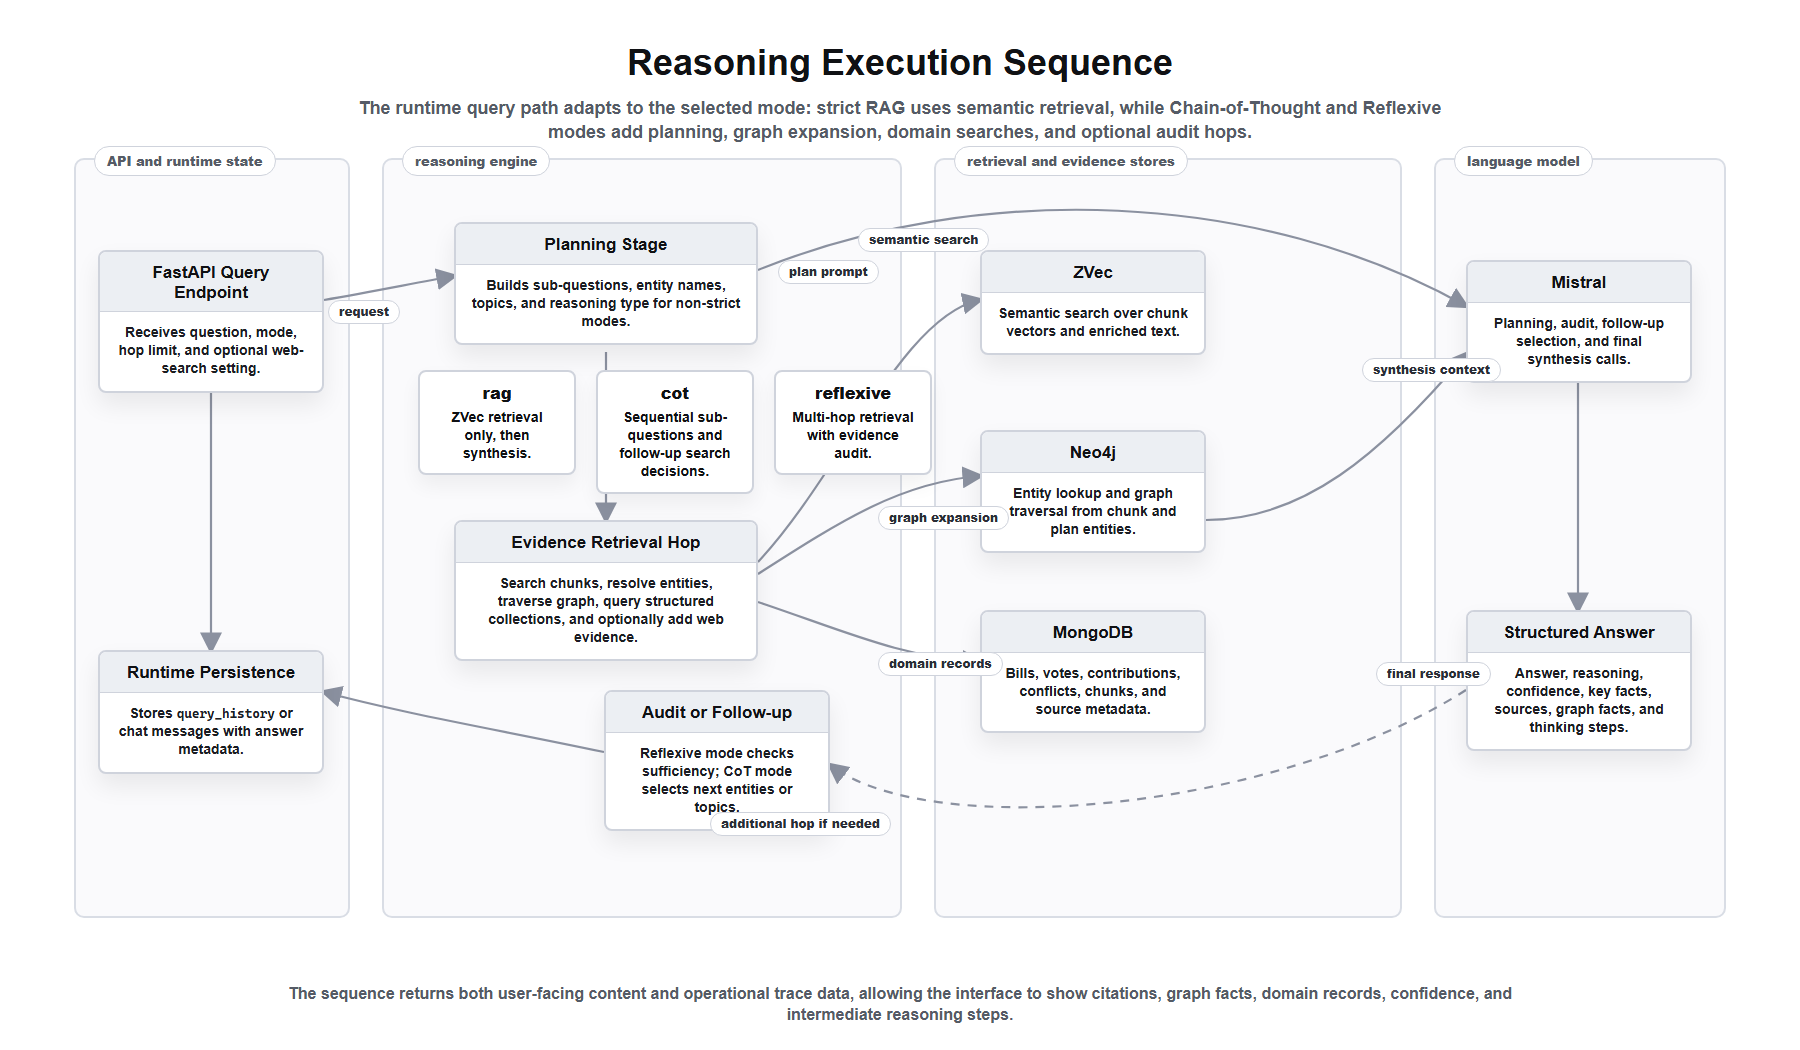
\includegraphics[width=0.96\textwidth,height=0.78\textheight,keepaspectratio]{images/sequence_reasoning.png}
    \caption{Reasoning execution sequence across retrieval, graph expansion, audit, and synthesis.}
    \label{fig:sequence-reasoning}
\end{figure}

Three modes are exposed at query time, trading latency against analytical depth. \textbf{Standard RAG (\texttt{rag})} performs one-hop semantic retrieval from ZVec using the user question, then direct synthesis; it suits factual lookups with minimal latency. \textbf{Chain-of-thought (\texttt{cot})} decomposes complex questions into sub-queries and may follow entities or topics across hops before synthesis. \textbf{Reflexive (\texttt{reflexive})} evaluates completeness and consistency after retrieval; insufficient evidence triggers refined retrieval rather than immediate answer generation. Mode selection implements FR-05 at architecture level; Chapter~4 details the \texttt{ReasoningEngine} and DSPy orchestration. Interface-level traces expose steps to satisfy FR-07 regardless of mode.

Evidence fusion merges ranked chunks, graph facts (nodes, edges, paths), and relevant structured records into a single context package for the synthesizer. Ranking considers semantic score, graph distance to seed entities, temporal validity, and deduplication of syndicated passages. Conflicting assertions are passed with provenance so synthesis can qualify claims rather than collapse contradictions silently. Fusion rules are mode-dependent: standard RAG prioritizes chunk relevance; multi-hop modes weight graph expansion; reflexive mode may narrow retrieval targets after audit feedback.

Figure~\ref{fig:technical-class-diagram} summarizes the logical service layering (API routes, domain services, store connectors, model clients) that implements the reasoning and ingestion designs above. Persistence access is isolated from orchestration logic so stores can be mocked or replaced during testing and evolution.

\begin{figure}[H]
    \centering
    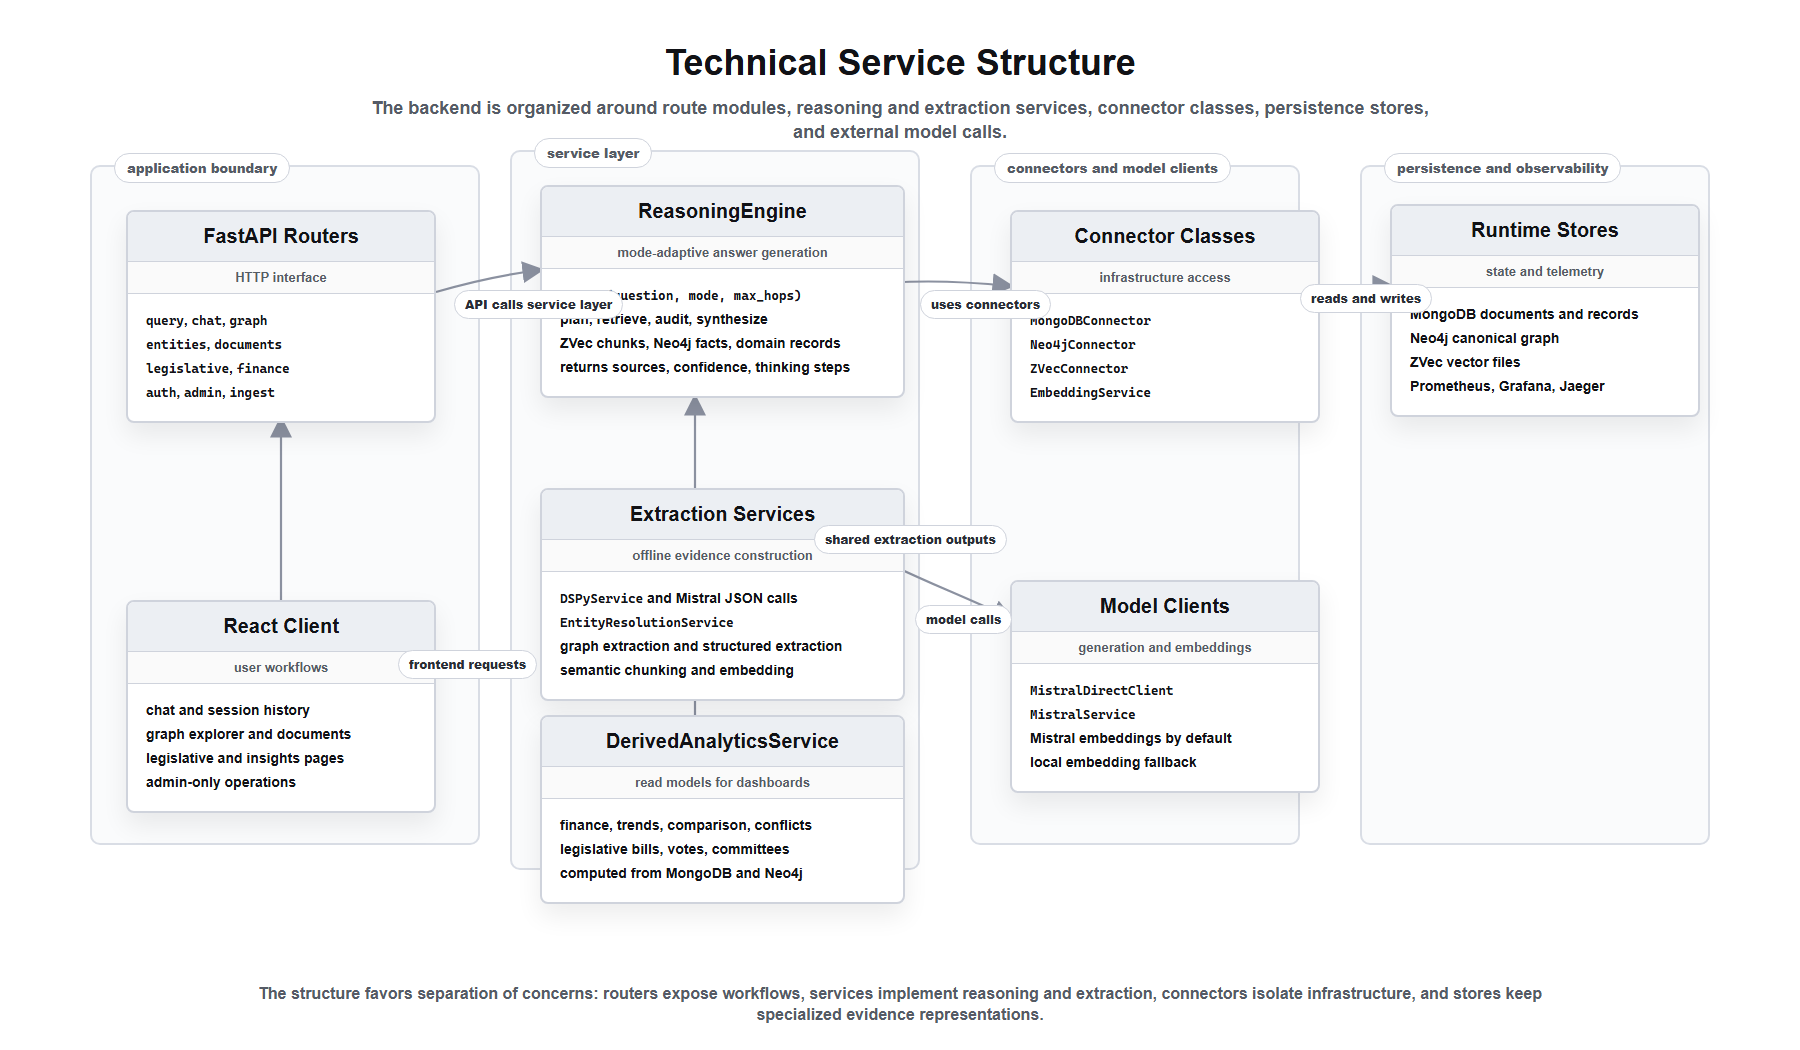
\includegraphics[width=0.96\textwidth,height=0.78\textheight,keepaspectratio]{images/technical_class_diagram.png}
    \caption{Technical service structure across API routes, services, connectors, stores, and model clients.}
    \label{fig:technical-class-diagram}
\end{figure}

\section{Conclusion}

This chapter specified the design of the political Graph-RAG platform: principles for modularity and traceability, refined use cases with access boundaries, offline and online data flows, multi-level ingestion with quality gates and state checkpoints, hybrid knowledge representation with temporal and provenance links, polyglot physical schemas, and a plan--retrieve--synthesize reasoning architecture with three selectable modes. The design directly addresses the functional and non-functional requirements of Chapter~2. Chapter~4 will describe how these structures are implemented in code, containers, and operational tooling; Chapter~5 will evaluate whether the resulting system meets the validation criteria in practice.
